\documentclass[12pt]{article}
 
\usepackage[margin=1in]{geometry}
\usepackage{amsmath,amsthm,amssymb}
\usepackage{mathtools}
\DeclarePairedDelimiter{\ceil}{\lceil}{\rceil}
%\usepackage{mathptmx}
\usepackage{accents}
\usepackage{comment}
\usepackage{graphicx}
\usepackage{IEEEtrantools}
 \usepackage{float}
 \usepackage{tikz-cd}
 
\newcommand{\N}{\mathbb{N}}
\newcommand{\Z}{\mathbb{Z}}
\newcommand{\R}{\mathbb{R}}
\newcommand{\Q}{\mathbb{Q}}
\newcommand*\conj[1]{\bar{#1}}
\newcommand*\mean[1]{\bar{#1}}
\newcommand\widebar[1]{\mathop{\overline{#1}}}


\newcommand{\cc}{{\mathbb C}}
\newcommand{\rr}{{\mathbb R}}
\newcommand{\qq}{{\mathbb Q}}
\newcommand{\nn}{\mathbb N}
\newcommand{\zz}{\mathbb Z}
\newcommand{\aaa}{{\mathcal A}}
\newcommand{\bbb}{{\mathcal B}}
\newcommand{\rrr}{{\mathcal R}}
\newcommand{\fff}{{\mathcal F}}
\newcommand{\ppp}{{\mathcal P}}
\newcommand{\eps}{\varepsilon}
\newcommand{\vv}{{\mathbf v}}
\newcommand{\ww}{{\mathbf w}}
\newcommand{\xx}{{\mathbf x}}
\newcommand{\ds}{\displaystyle}
\newcommand{\Om}{\Omega}
\newcommand{\dd}{\mathop{}\,\mathrm{d}}
\newcommand{\ud}{\, \mathrm{d}}
\newcommand{\seq}[1]{\left\{#1\right\}_{n=1}^\infty}
\newcommand{\isp}[1]{\quad\text{#1}\quad}
\newcommand*\diff{\mathop{}\!\mathrm{d}}

\DeclareMathOperator{\imag}{Im}
\DeclareMathOperator{\re}{Re}
\DeclareMathOperator{\diam}{diam}
\DeclareMathOperator{\Tr}{Tr}
\DeclareMathOperator{\cis}{cis}

\def\upint{\mathchoice%
    {\mkern13mu\overline{\vphantom{\intop}\mkern7mu}\mkern-20mu}%
    {\mkern7mu\overline{\vphantom{\intop}\mkern7mu}\mkern-14mu}%
    {\mkern7mu\overline{\vphantom{\intop}\mkern7mu}\mkern-14mu}%
    {\mkern7mu\overline{\vphantom{\intop}\mkern7mu}\mkern-14mu}%
  \int}
\def\lowint{\mkern3mu\underline{\vphantom{\intop}\mkern7mu}\mkern-10mu\int}




\newenvironment{theorem}[2][Theorem]{\begin{trivlist}
\item[\hskip \labelsep {\bfseries #1}\hskip \labelsep {\bfseries #2.}]}{\end{trivlist}}
\newenvironment{lemma}[2][Lemma]{\begin{trivlist}
\item[\hskip \labelsep {\bfseries #1}\hskip \labelsep {\bfseries #2.}]}{\end{trivlist}}
\newenvironment{exercise}[2][Exercise]{\begin{trivlist}
\item[\hskip \labelsep {\bfseries #1}\hskip \labelsep {\bfseries #2.}]}{\end{trivlist}}
\newenvironment{problem}[2][Problem]{\begin{trivlist}
\item[\hskip \labelsep {\bfseries #1}\hskip \labelsep {\bfseries #2.}]}{\end{trivlist}}
\newenvironment{question}[2][Question]{\begin{trivlist}
\item[\hskip \labelsep {\bfseries #1}\hskip \labelsep {\bfseries #2.}]}{\end{trivlist}}
\newenvironment{corollary}[2][Corollary]{\begin{trivlist}
\item[\hskip \labelsep {\bfseries #1}\hskip \labelsep {\bfseries #2.}]}{\end{trivlist}}

\newenvironment{solution}{\begin{proof}[Solution]}{\end{proof}}
 
\begin{document}
 
% --------------------------------------------------------------
%                         Start here
% --------------------------------------------------------------
\title{Math 120TC Homework 5}
\author{Ethan Martirosyan}
\date{\today}
\maketitle
\hbadness=99999
\hfuzz=50pt
\section*{Problem 1}
First, we note that \[K_5 = \{\{1\},\{2\},\{3\},\{4\},\{5\},\{1,2\},\{1,3\},\{1,4\},\{1,5\},\{2,3\},\{2,4\},\{2,5\},\{3,4\},\{3,5\},\{4,5\}\}\] Since $V((K_{5})_\Delta^{*2}) = V(K_5) \sqcup V(K_5)$, we know that $\vert V((K_{5})_\Delta^{*2}) \vert = 10$. We may suppose that $5$ of the vertices are in $\rr^5$ at the vectors $e_1$, $e_2$, $e_3$, $e_4$, and $e_5$. Then, there is a $4$ dimensional hyperplane going through these five vectors, so we may consider them to be in $\rr^4$. Then, their negatives would be the other $5$ vertices. Now, we will determine the geometric nature of $(K_{5})_\Delta^{*2}$. We claim that it is the boundary of a convex $4$-polytope in $\rr^4$. Let us write the 10 vertices as follows:
\[
\{1\},\{2\},\{3\},\{4\},\{5\},\{-1\},\{-2\},\{-3\},\{-4\},\{-5\}
\] Notice that the vertex $1$ is connected to $8$ vertices; namely, the $8$ vertices that aren't $1$ or $-1$. Let us examine the link at $1$. If we look at the vertex $2$, we note that the link contains 
\[
\{\{2\}, \{2,-3\}, \{2,-4\}, \{2,-5\}, \{2,-3,-4\}, \{2,-3,-5\}, \{2,-4,-5\}\}
\] From this alone, we find that the link contains $2$ complexes. We deduce that the boundary near the vertex $1$ is a $3$ dimensional object. Furthermore, this holds for every other vertex as well so that the deleted product $(K_5)^{*2}_{\Delta}$ must be the boundary of a convex $4$ polytope. Let us examine this some more. Consider the below image:
\begin{figure}[H]
\centering
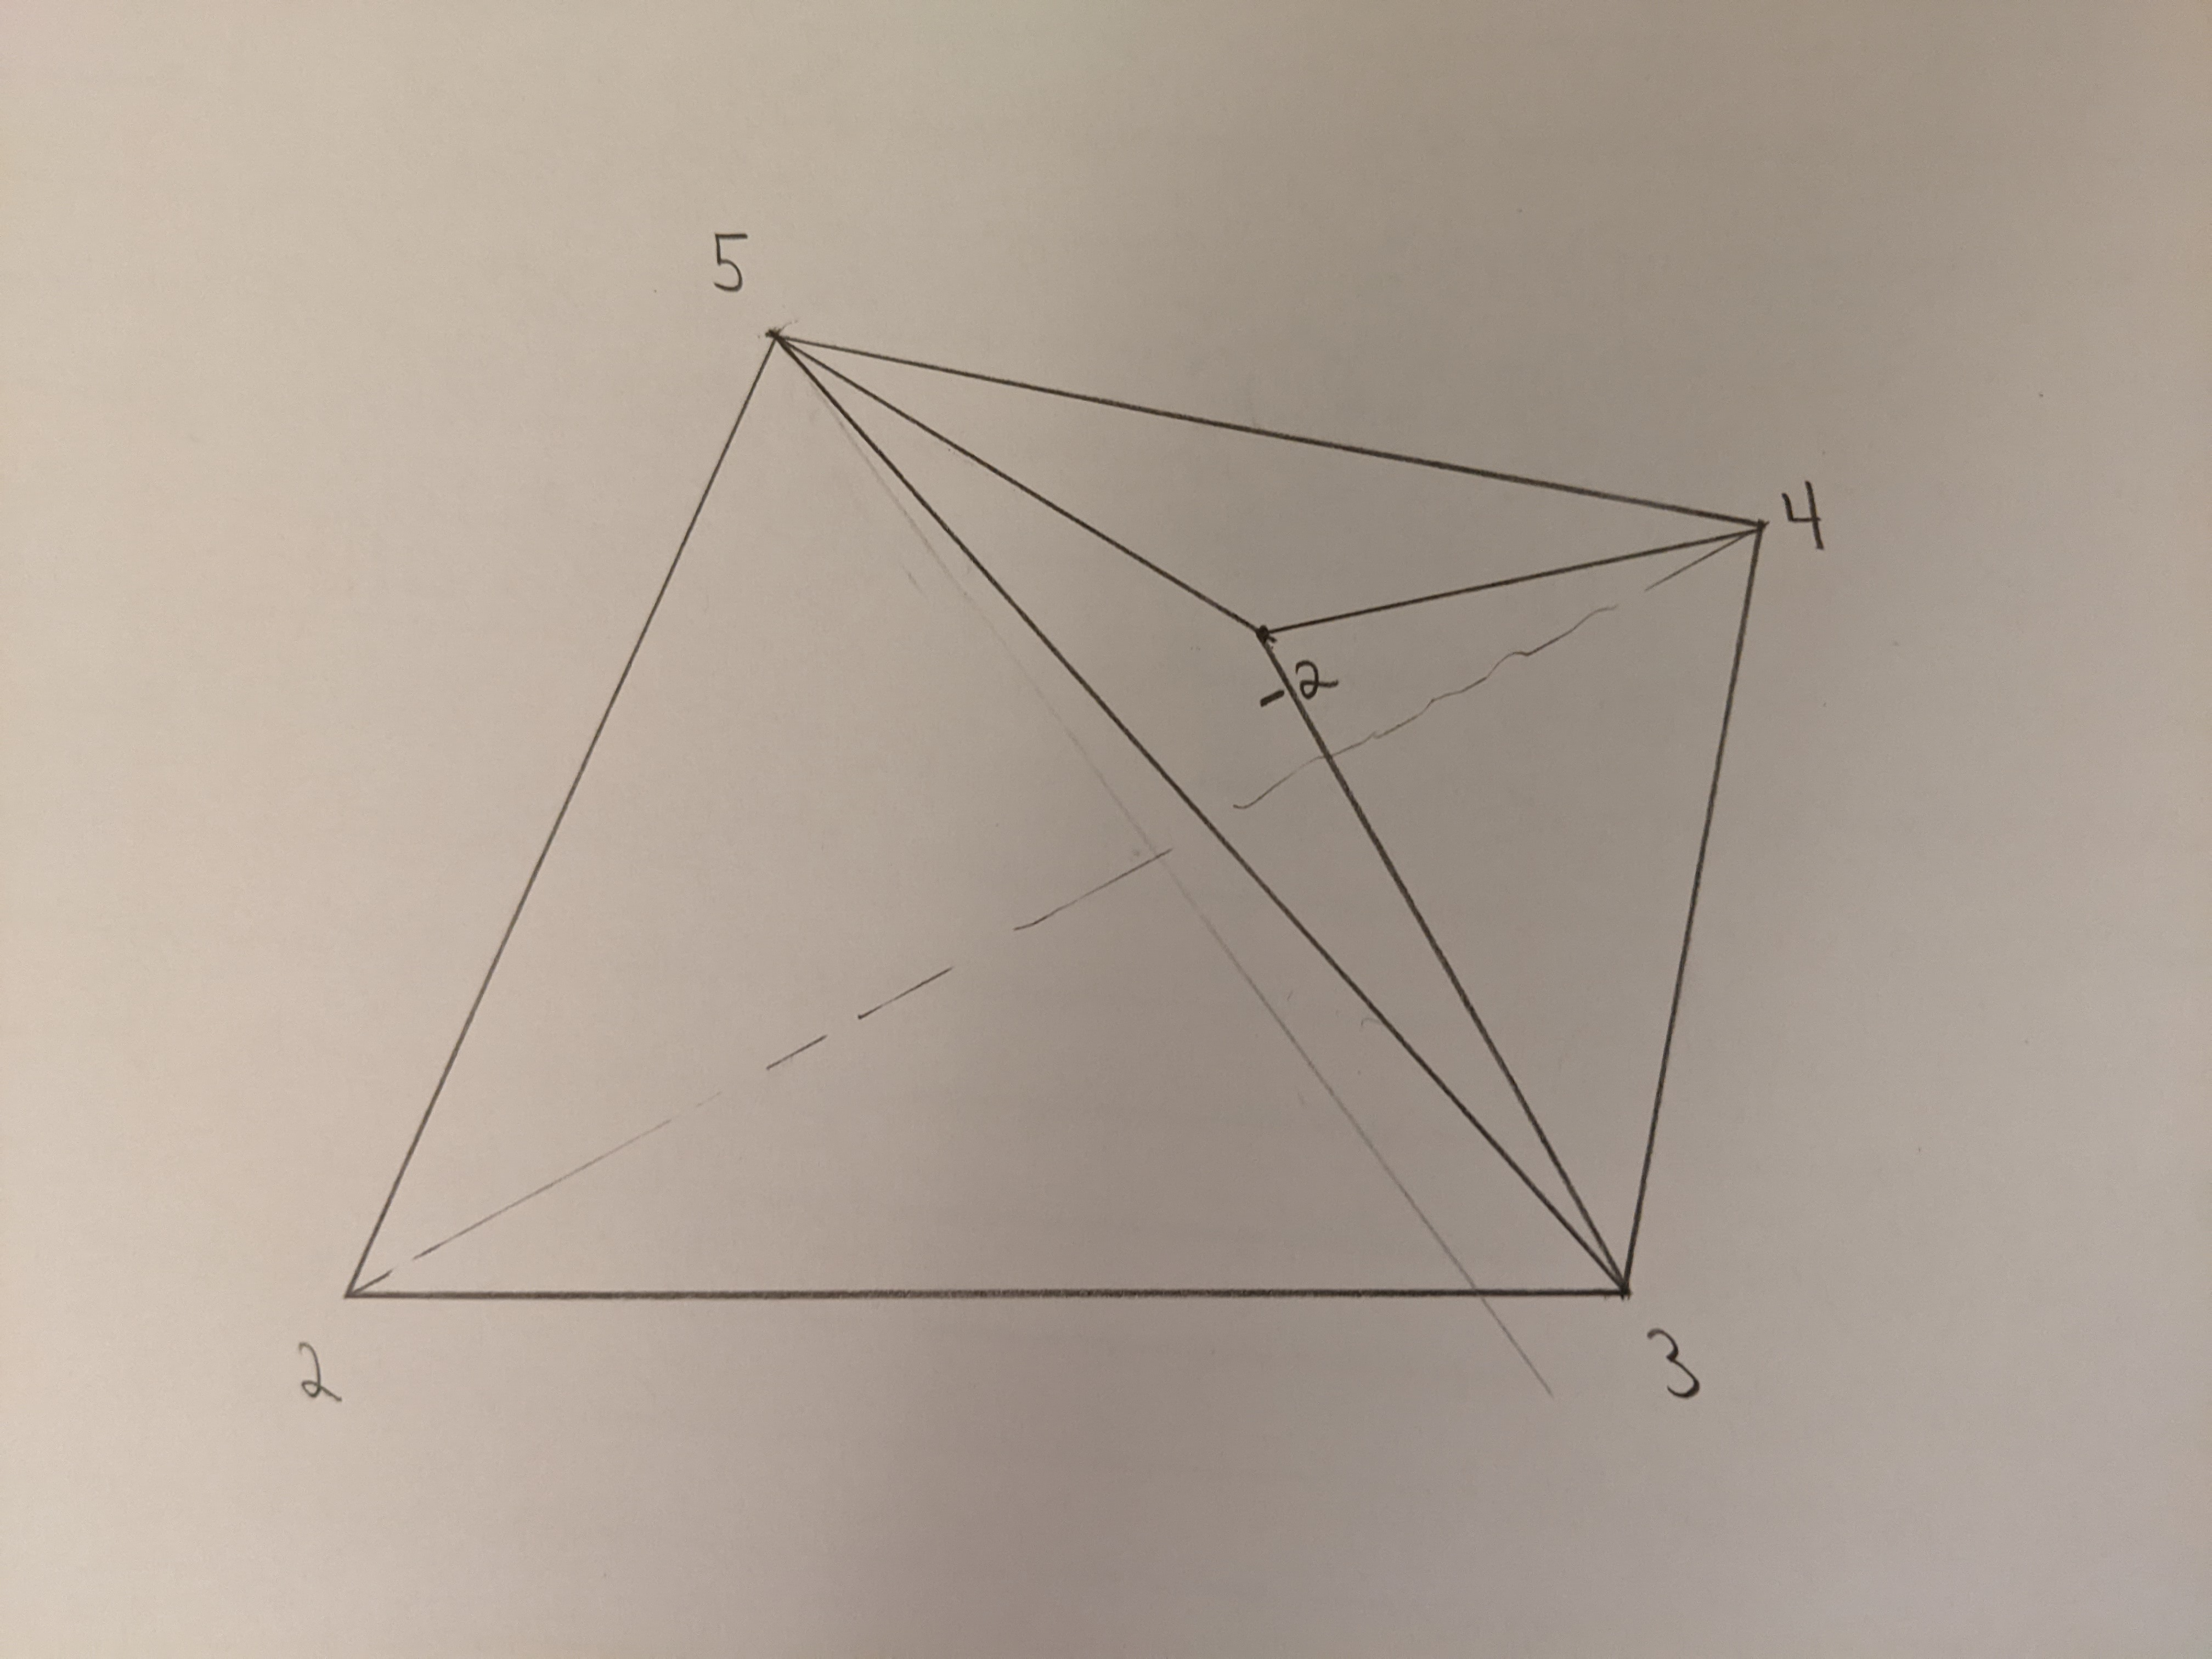
\includegraphics[width=\textwidth]{Image1}
\end{figure}
In this picture, we have drawn the simplex corresponding to $2,3,4,5$. In accordance with our notation, we have put $-2$ on the opposite side and connected it to $3,4,5$. From this picture, it is evident that the deleted join cannot be embedded into $3$ space and that it must be in $4$ space at least. This provides more evidence to support the assertion that the deleted join is the boundary of a $4$ polytope. Just to be certain, we compute the deleted product below:
\begin{figure}[H]
\centering
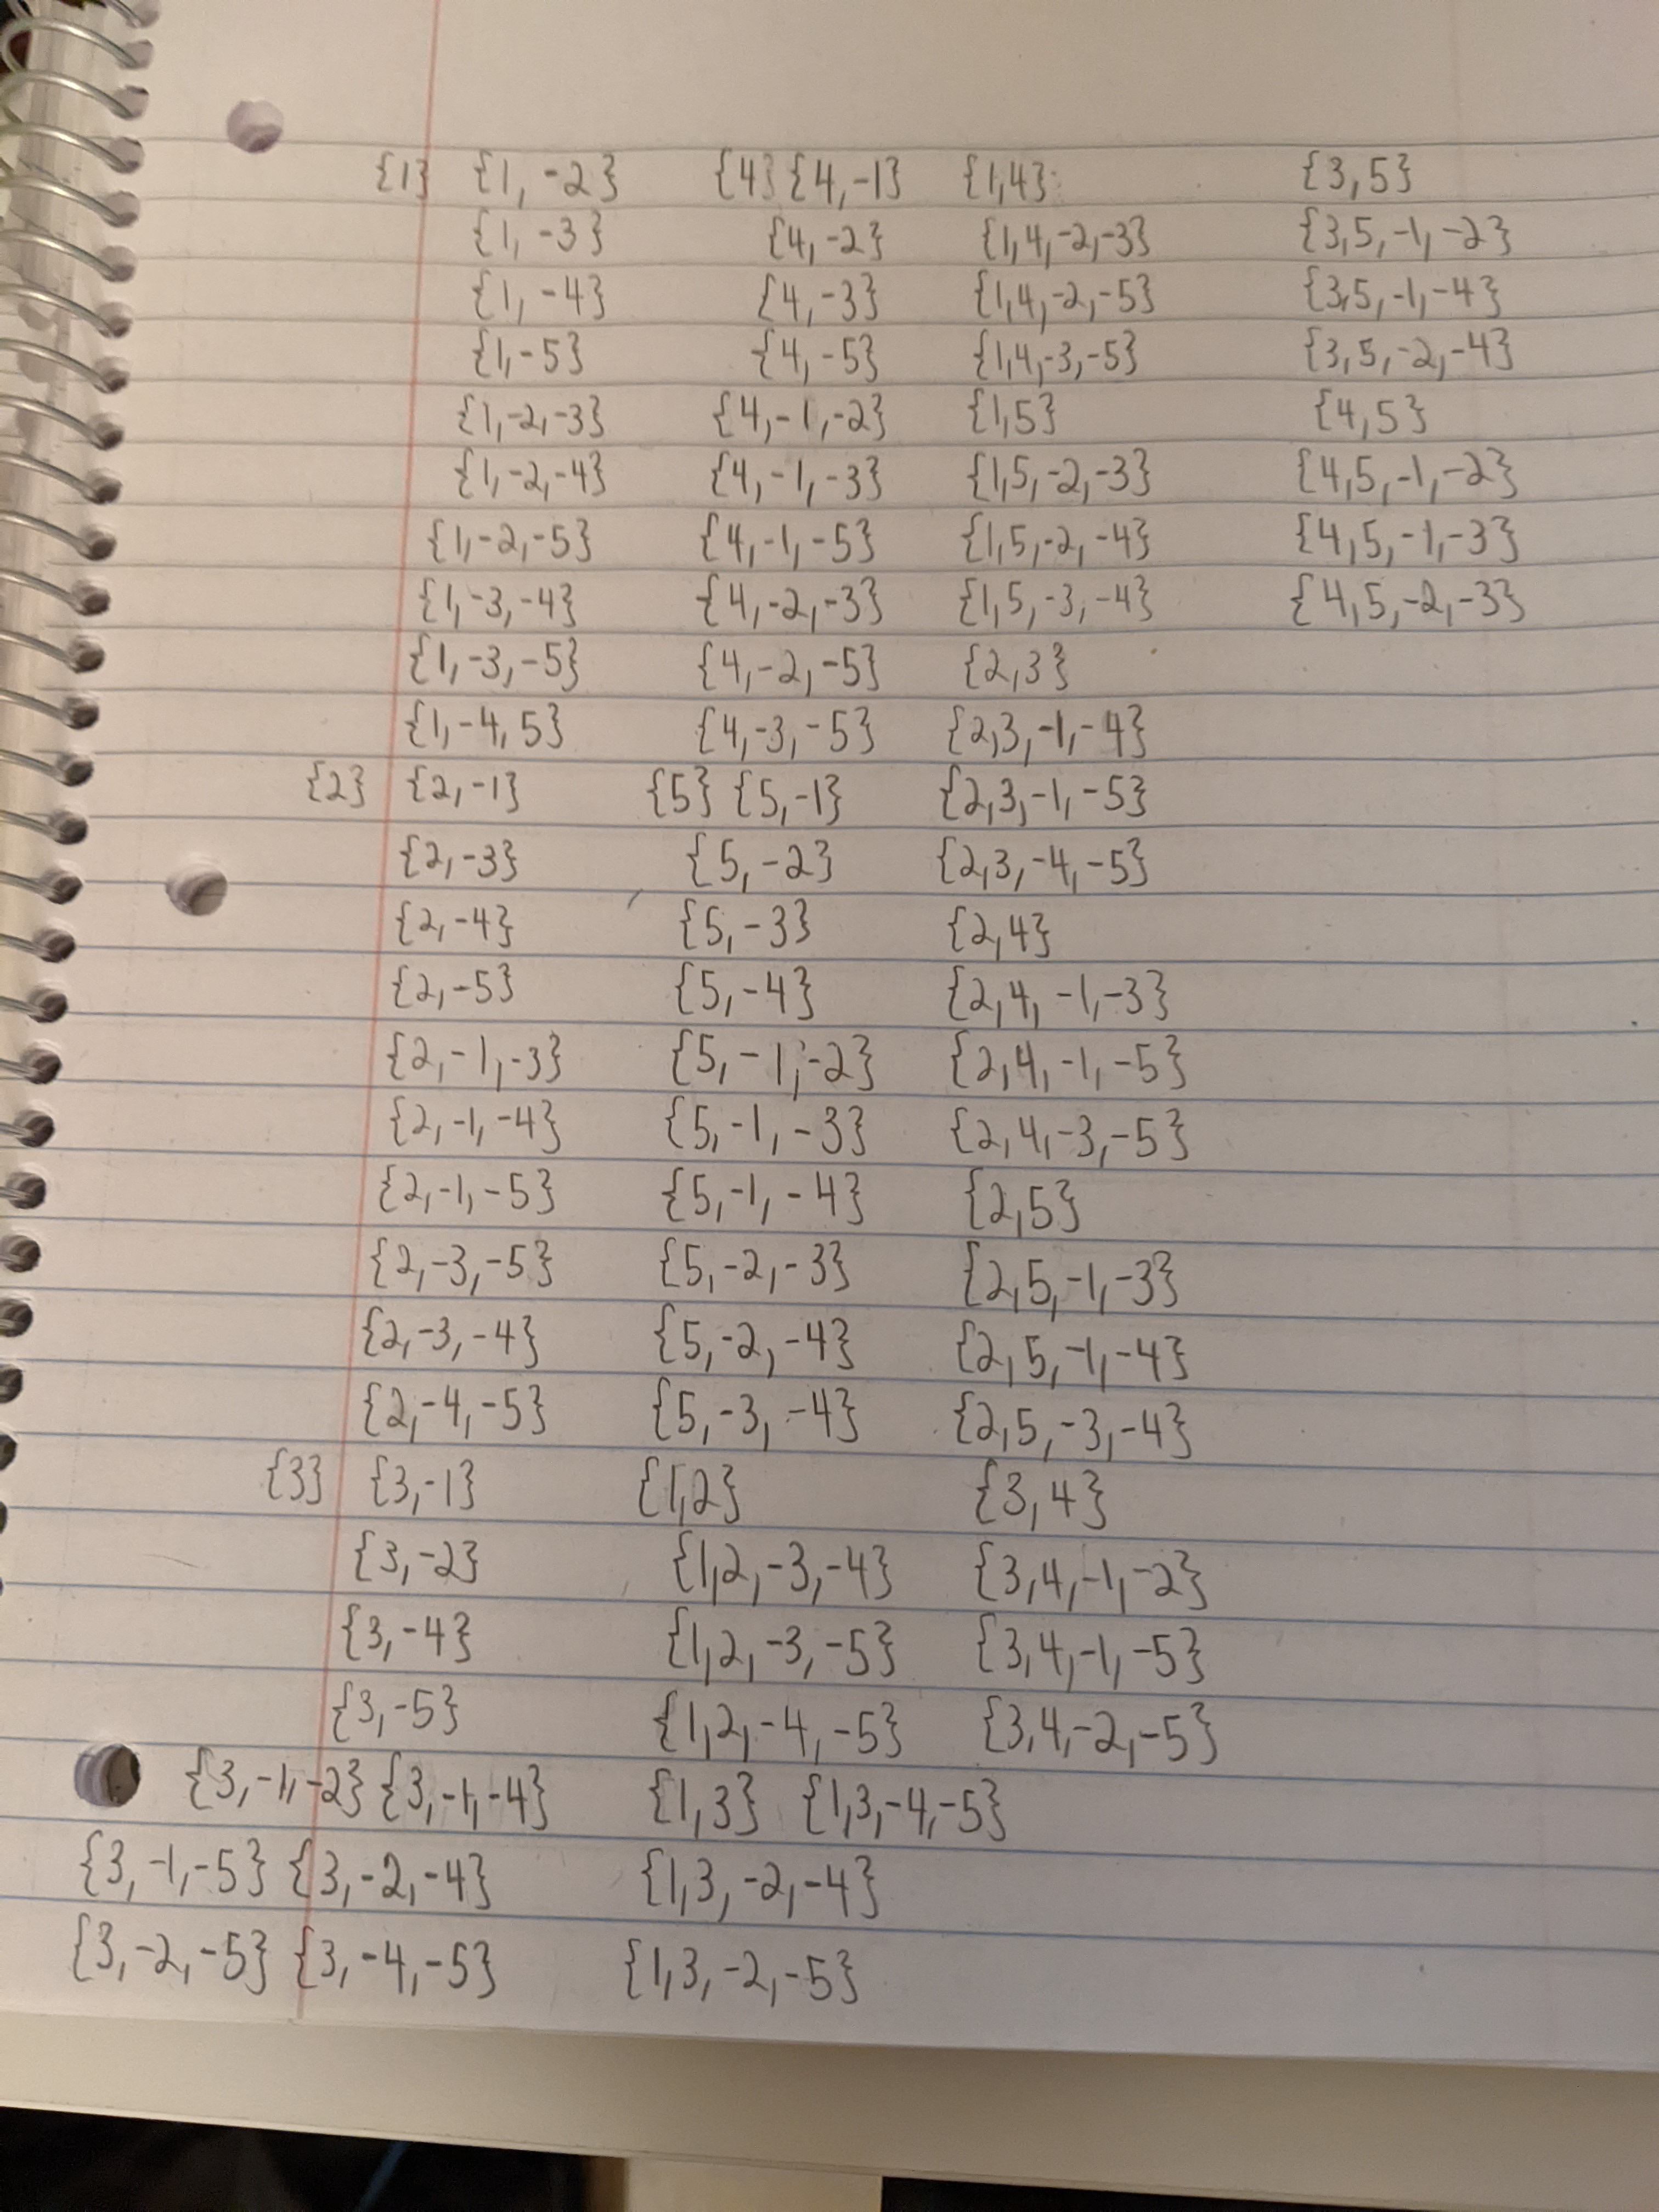
\includegraphics[width=\textwidth]{Image2}
\end{figure}
\newpage
\section*{Problem 2}
Let $f: S^k \rightarrow S^n$ and $g: S^\ell \rightarrow S^n$ be odd maps. Then, we know that the following diagrams commute:
\[ \begin{tikzcd}
S^k \arrow{r}{f} \arrow[swap]{d}{\nu} & S^n \arrow{d}{\nu} \\%
S^k \arrow{r}{f}& S^n
\end{tikzcd}
\] and
\[ \begin{tikzcd}
S^\ell \arrow{r}{g} \arrow[swap]{d}{\nu} & S^n \arrow{d}{\nu} \\%
S^\ell \arrow{r}{g} & S^n
\end{tikzcd}
\] where $\nu$ represents the antipodality map on $S^k$, $S^\ell$, or $S^n$ (that is, we have $f(-x) = -f(x)$ and $g(-x) = - g(x)$). Now, we have a map $f * g: S^k * S^\ell \rightarrow S^{n} * S^{n}$ given by $f * g(x,y,t) = (f(x),g(y),t)$. Let us assume that $f(S^k) \cap g(S^\ell) = \varnothing$. Then, we know that $f * g$ maps $S^k * S^\ell$ into $(S^n)^{*2}_{\Delta}$, that is, the deleted join of $S^n$ considered as a space. As in Lemma $5.5.4$, we can construct a $\zz_2$-map from $(S^n)^{*2}_{\Delta} \rightarrow S^n$ so that $\text{ind}_{\zz_2}((S^n)^{*2}_{\Delta}) \leq n$. However, we know that $S^k * S^\ell$ is homeomorphic to $S^{k+\ell+1}$ so that $\text{ind}_{\zz_2}(S^k * S^\ell) = k+\ell+1 \geq n + 1$. Thus, we have reached a contradiction, and we know that $f(S^k) \cap g(S^\ell) \neq \varnothing$. 
\end{document} 